\documentclass[a4paper, 11pt]{article}

\usepackage{amsmath, amssymb, amstext, amsfonts, mathrsfs}  % Mathe
\usepackage{hyperref}       %Anklicken von Links
\usepackage[normalem]{ulem} %weitere Formatierung von Schriften
\usepackage{fancyhdr}       %sch\"one Kopf- und Fußzeilen
\usepackage{verbatim}
\usepackage{graphicx}
\usepackage{pgfplotstable}
\usepackage{booktabs} % required for using tables
\usepackage{float}
\usepackage{listings}
\usepackage{xcolor}

\definecolor{codegreen}{rgb}{0,0.6,0}
\definecolor{codegray}{rgb}{0.5,0.5,0.5}
\definecolor{codepurple}{rgb}{0.58,0,0.82}
\definecolor{backcolour}{rgb}{0.95,0.95,0.92}

\lstdefinestyle{mystyle}{
    backgroundcolor=\color{backcolour},   
    commentstyle=\color{codegreen},
    keywordstyle=\color{magenta},
    numberstyle=\tiny\color{codegray},
    stringstyle=\color{codepurple},
    basicstyle=\ttfamily\footnotesize,
    breakatwhitespace=false,         
    breaklines=true,                 
    captionpos=b,                    
    keepspaces=true,                 
    numbers=left,                    
    numbersep=5pt,                  
    showspaces=false,                
    showstringspaces=false,
    showtabs=false,                  
    tabsize=2
}
\lstset{style=mystyle}

\pagestyle{fancy}
\lhead{Data-driven intelligent systems\\}
\chead{\ \\Florian Vahl, Dominik Buchhardt}
\rhead{\today\\}

\parindent0pt

\pgfplotstableset{% global config, for example in the preamble
  every head row/.style={before row=\toprule, after row=\midrule},
  every last row/.style={after row=\bottomrule},
  fixed,precision=3,
}

\begin{document}

\section{Markov Decision Process}
\subsection{Description}
The Markov decision process is a process where the action of an agent only depends on the current state of the environment.
There are is a set of possible actions and a set of possible states. There is also an agent policy which choses an action based on the given state.
The agent receives information about the state, performs the action provided by its policy and may receives a reward for the action. The state is updated and executed another time.
The MPD has fixed transition probabilities which depend as said only on the current state.
The reward probability is also fixed.

The agents policy will be adapted to gain a maximum Return meaning a maximum future reward.
The reward is estimated by estimating the Return for the next step and adding the reward for the transition.

The best estimates for this transition are stored as $V$ values depending on the state or $Q$ depending on both the state and the action.

\subsection{Example for a MDP}

A robot navigates through a maze, the states are the positions and orientations of the robot.
The actions are the movement commands. The reward is given based on the proximity to the goal position.


\subsection{Example for a POMPD}

A real life application where the robot from above is only able to measure a few of the values which are defining its state.
Therefore it is only able to approximate a distribution of possible states and apply a more general form of the MDP.

\section{Exploration vs. exploitation}

In reinforcement learning exists a tradeoff between exploration and exploitation.
Exploitation means optimizing the currently best working policy towards a local maximum.
Exploration on the other hand means trying out new or worse strategies to explore unknown states and skip local maxima in the best case towards a global maximum.
\\\\
This tradeoff can be implemented using a $\epsilon$-greedy action selection, where a random action is chosen with a probability of $1-\epsilon$ for exploration purposes.
If no random action is selected the currently best fitting action is chosen.
\\\\
An agent may be failing or take a very long time to converge if it explores too much.
On the other hand, exploiting too much results in a local maximum of the reward, meaning it maybe fails to choose an action that is suboptimal at the moment but leads to a much higher reward later on.

\section{SARSA and Q-Learning}
\subsection{is temporal difference (TD) learning?}
TD Learning is a class of model-free reinforcement learning methods. TD learning adjusts the estimated Return every few steps (e.g. every step) instead of waiting for a final Outcome. TD-learning can be used in combination with Neural Networks to optimize the adjusting of the estimates.

\subsection{How does the SARSA algorithm work?}
The SARSA Algorithm is a TD-Learning method. The Algorithm is used again and again with many initial states to learn the entire state space well.\\
SARSA initializes a Round (Trial) by selecting an Action a for an initial State s und calculating the corresponding Q-Value. Next it repeats until the Round is over when e.g. the final State is reached or it got Out-Of-Bounds. Next it executes the selected Action a, reads the Reward r and the reached State s' and selects the next Action with the current Target Policy. It calculates the TD-Error for this iteration from the State s, the Action a, the Reward r obtained from this transition, the next State s' and the next Action a', hence the acronym SARSA. The Q-Value for the State s and Action a is updated with the previously calculated TD-Error.
It provides the latest Values for the next Iteration by updating the Variables Q(s, a), s and a with the Values of Q(s', a'), s' and a'.

\subsection{How does Q-learning work, and how is it different from SARSA?}
Q-Learning works exactly the same as SARSA except that the TD-Error is calculated differently. SARSA is a On-Policy Algorithm as it uses the actually selected Action and State from the Policy for calculating the Q-Value. 
Q-Learning is an Off-Policy Algorithm instead and uses the best possible Q-Value for all next Actions and States instead of the ones selected by the Target Policy.

\section{Implementing Q-Learning}
The values in the Q-Table describe the estimated Return for taking a specific Action in a specific State/Observation. Looking at the output summary of q\_table it seems that dropping passengers is penalized compared to moving around and picking passengers up which is expected as dropping an passenger on a invalid field is penalized with a Reward of -10. \\
The updated Code:\\
\begin{lstlisting}[language=Python]
# This is the main loop.
num_train_episodes = 1000  # Modify to tune for convergence
render = True  # Set to False to speed up training
returns = []
# This creates our Q-table: A two-dimensional array of all zeros.
q_table = np.zeros([num_observations, num_actions])
print('Shape of the Q-table:', q_table.shape)

def best_action(observation):
    q_value, action = float("-inf"), -1

    actions = q_table[observation]

    for a, q in enumerate(actions):
        if q > q_value:
            q_value = q
            action = a

    # select best action with epsilon greed policy
    best_probability = 1 - epsilon
    other = epsilon / (num_actions - 1)
    
    probabilities = []
    
    for a in range(num_actions):
        if a == action:
            p = best_probability
        else:
            p = other
        probabilities.append(p)

    action = np.random.choice(list(range(num_actions)), p=probabilities)

    # return the action and its current q_value for the given state
    return action, actions[action]

for episode in range(1, num_train_episodes):
    # By resetting the environment you also 
    # get the initial observation or "state".
    observation = env.reset()

    # Repeat until the environment is done.
    done = False
    episode_return = 0
    
    # ME: select best action for initial state with epsilon-greedy
    action, q_value = best_action(observation) 
    
    while not done:
        # Perform the chosen action in the environment 
        # to get reward values and the next observation.
        next_observation, reward, done, _ = env.step(action)
        
        # Update your Q-table based on the information you gathered!
        next_action, next_q_value = best_action(next_observation) 
        
        # ME: calculate the td_error depending 
        # on the maximum q_value for the next state
        best_next_q = np.max(q_table[next_observation])
        td_error = reward + (gamma * best_next_q) - q_value
        # ME: update the q_table for the current state and action
        q_table[observation, action] = q_value + (alpha * td_error)
        
        # Step the observation
        observation = next_observation
        # ME: update action
        action = next_action
        # ME: update q_value
        q_value = next_q_value
                
        # For performance reasons, only display every 200th episode.
        episode_return += reward
        if render and episode % 200 == 0:
            clear_output(wait=True)
            env.render()
            print("Episode: ", episode)
            print("Reward: ", reward)
            print("Return so far: ", episode_return)
            # Wait a little bit. We don't want to go too fast.
            sleep(0.1)
    returns.append(episode_return)
\end{lstlisting}
\begin{figure}
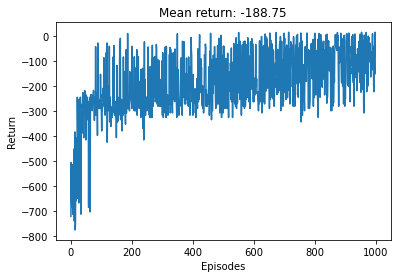
\includegraphics{1000_iterations.png}
\caption{1000 Episodes. In the first 100 Episodes the Return increases dramatically and slows down afterwards. It does not seem to converge yet.}
\end{figure}
\begin{figure}
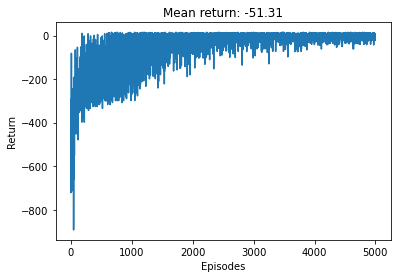
\includegraphics{5000_iterations.png}
\caption{5000 Episodes. It does not seems to converge around zero which is expected as the maximum Return is at most 20 for dropping the passenger (if picking up and dropping happens on the same field).}
\end{figure}
\begin{figure}
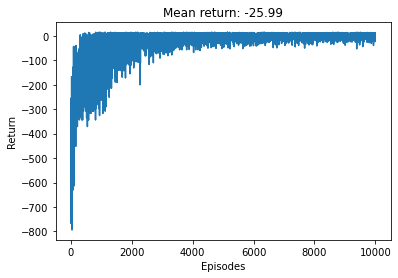
\includegraphics{10000_iterations.png}
\caption{10000 Episodes. No major improvements are seen compared to 5000 Episodes. The Agent seems to have converged.}
\end{figure}
\end{document}
